\documentclass[11pt]{article}
\usepackage{amsmath,graphicx,hyperref,booktabs,longtable}
\newcommand\project[1]{Project \textsc{#1}}
\title{A Native LaTeX Import Study}
\author{Ada Lovelace \and Grace Hopper}
\date{June 2026}

\begin{document}
\maketitle

\begin{abstract}
This article tests a semantic import path for \project{Harbor}. It keeps
\emph{meaningful structure} editable instead of reproducing page layout.
\end{abstract}

\tableofcontents

\section{Methods}\label{sec:methods}
The method uses \textbf{native PHP} and links to
\href{https://example.test/method}{the implementation note}. A footnote keeps
context\footnote{Footnotes become WordPress note references.} close to its text.

The energy estimate is $E = mc^2$.

\begin{equation}
  \alpha + \beta = \gamma
  \label{eq:identity}
\end{equation}

\begin{align}
  f(x) &= x^2 + 1 \\
  g(x) &= \frac{1}{x}
\end{align}

\begin{itemize}
  \item Preserve headings, labels, and links.
  \item Keep \texttt{inline code} as code.
\end{itemize}

\begin{enumerate}
  \item Parse source safely.
  \item Never execute TeX packages or shell escapes.
\end{enumerate}

\begin{quote}
Editable structure is more useful than a simulated printed page.
\end{quote}

\begin{figure}
  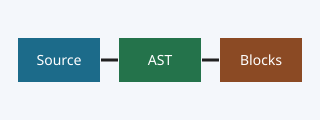
\includegraphics[width=0.5\textwidth]{figures/architecture.svg}
  \caption[Architecture]{The import architecture.}
  \label{fig:architecture}
\end{figure}

\begin{table}
  \caption{Import quality gates.}
  \label{tab:gates}
  \begin{tabular}{lcr}
    \toprule
    Gate & Scope & Status \\
    \midrule
    Text & Paragraphs & Ready \\
    Media & Figures & Ready \\
    \bottomrule
  \end{tabular}
\end{table}

As shown in \autoref{fig:architecture}, the table in \ref{tab:gates} supports
the method in \ref{sec:methods}. Equation \ref{eq:identity} remains math.
\citep[pp. 12--14]{knuth1984,lamport1994}

\subsection{Imported Appendix}\label{sec:appendix}
The local include is parsed through a bounded PHP file resolver. Unknown
commands such as \custompublisher{review} remain visible raw TeX instead of
being executed or discarded.


\bibliographystyle{plain}
\bibliography{references}
\end{document}
